\chapter{DCF77}
\section{Inleiding}
In dit onderdeel, genaamd DCF77,  wordt de basis van de wekker gelegd, door verschillende belangrijke datasignalen aan te maken, welke nodig zijn om de rest van de wekker goed te laten functioneren. Een eis die is gesteld aan de eigenschappen van deze klok, is dat deze gesynchroniseerd wordt met het zogenaamde DCF77 signaal. Dit is een signaal dat vanuit Duitsland wordt verzonden en bestaat uit korte (100 ms) en lange (200 ms) pulsen, welke respectievelijk nullen en enen coderen. Iedere seconde, behalve de laatste van iedere minuut, wordt er een puls verzonden. De bits die door deze pulsen worden gecodeerd, bevatten allerlei informatie, zoals de actuele datum en tijd op de eerstvolgende minuut. Een deel van de informatie die op deze manier wordt verzonden, zal worden gebruikt voor het aansturen van de wekker. Om gebruik te kunnen maken van de informatie die met het DCF77 signaal wordt verzonden, is het echter wel nodig te weten welke bit uit de reeks van 59 stuks welke informatie codeert. In figuur \ref{fig:dcfsignaal} is te zien welke informatie door elk van de 59 bits wordt gecodeerd. Een versie in tabelvorm is te vinden op Wikipedia ~\cite{Tijdwiki}. De wekker zal gebruik gaan maken van bits 21 t/m 58. In de afbeelding worden binnen deze selectie bits 28, 35 en 58 respectievelijk P1, P2 en P3 genoemd. Deze bits zijn zogenaamde parity-bits, welke de ontvanger van het DCF77 signaal in staat stelt om tot op zekere hoogte te controleren of de ontvangen bitreeks correct is. In het DCF77 signaal wordt gebruik gemaakt van even parity. Dit betekent dat, wanneer zich in de bits die bij een zekere parity bit horen een even aantal logische enen bevindt, de parity bit een logische 0 zal zijn ~\cite{Tijdscodering}. Het DCF77 blok converteert een gedigitaliseerde versie van het DCF77 signaal naar een tijdreferentie, waarna deze een autonome klok synchroniseert, welke zich ook binnen het DCF77 blok bevindt.

\begin{figure}[h!]
\center
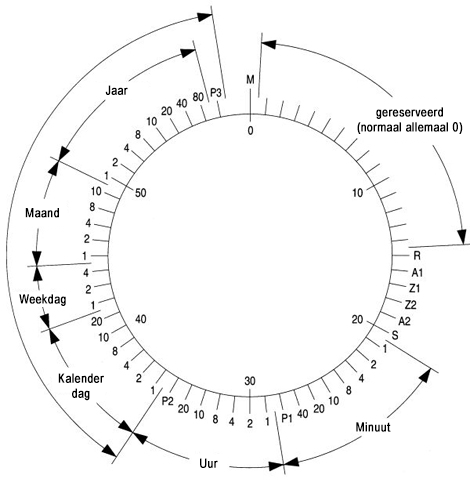
\includegraphics[scale=1.9]{Figuren/DCF77/dcf77coding.png}
\caption{Codering van het dcf-signaal~\cite{Tijdscodering}}
\label{fig:dcfsignaal}
\end{figure}

\section{Specificaties}
In deze sectie worden de in- en uitgangen van de DCF-controller overzichtelijk weergeven. Doordat dit onderdeel aan het begin staat van het totale systeem, bevat dit blok enkel standaard ingangen en een ingang van buitenaf met het DCF77 signaal. De uitgangen uren en minuten worden doorgestuurd naar de main-controller. De clk van 1 Hz zal in verschillende onderdelen worden gebruikt, zowel binnen als buiten het DCF77 blok. De datum en het signaal dcf\_led zullen rechtstreeks op het LCD scherm worden weergegeven. Enkele signalen zijn in BCD (Binairy Coded Decimal). Meer informatie over BCD is te vinden op ~\cite{BCDinfo}.

\subsection{Ingangen}
Dit onderdeel maakt gebruik van de volgende ingangen: 
\begin{itemize}[nolistsep]
\item De 32 kHz systeemklok, een standaard input.
\item Het 'active high' resetsignaal, een standaard input.
\item Het gedigitaliseerde DCF77 signaal, bestaande uit korte en lange pulsen.
\end{itemize}
\noindent

\subsection{Uitgangen}
Dit onderdeel genereert de volgende uitgangen:
\begin{itemize}[nolistsep]
\item Een kloksignaal met een frequentie van 1 Hz, welke gebruikt kan worden om secondes te tellen.
\item Het debug signaal dcf\_led, wat een seconde lang hoog is na ontvangst van een puls van het DCF77 signaal.
\item Uren; de uren van de huidige tijd in een BCD vector van 6 bits.
\item Minuten; de minuten van de huidige tijd in een BCD vector van 7 bits.
\item Weekdag; de dag van de week, binair gecodeerd met maandag als 001.
\item Dag; de dag van de maand in een BCD vector van 6 bits.
\item Maand; het nummer van de maand in een BCD vector van 5 bits.
\item Jaar; de laatste twee cijfers van het jaartal in een BCD vector van 8 bits.
\item Date\_ready; een signaal dat aangeeft dat de datum gereed is voor verder gebruik.
\end{itemize}

\subsection{Gedrag}
Het DCF77 blok heeft als belangrijkste gedragsfunctie om de huidige tijd en datum door te geven. Om deze informatie zo precies mogelijk te houden, dient deze zo vaak mogelijk te worden gesynchroniseerd met het extern gedigitaliseerde DCF77 ingangssignaal. Idealiter zou er dus iedere minuut met het DCF77 signaal worden gesynchroniseerd. Pas als via de parity bits is gebleken dat het de ontvangen tijd en datum plausibel zijn, wordt dit echter gedaan. Anders blijft de datum onveranderd en wordt de tijd bijgehouden met een interne klok. Zo wordt voorkomen dat andere onderdelen op de chip tijdelijk een compleet verkeerd signaal krijgen doorgestuurd, indien het DCF-signaal signaal niet of slecht wordt ontvangen.\\

\noindent Naast deze belangrijkste functie, heeft het DCF77 blok ook nog enige kleinere taken. Zo dient het 1 Hz signaal dat afkomstig is uit een interne klokdeler en wordt gebruikt voor de interne klok ook beschikbaar te worden gesteld voor gebruik in andere blokken. Ook dient een debug signaal dcf\_led gegenereerd te worden, dat na iedere ontvangen bit uit het DCF77 signaal een seconde lang hoog is. Ten slotte dienen alle subblokken, inclusief registers, van de gehele module bij een 'active high' reset gereset te worden.

\section{Functionaliteit}
Het DCF blok dient volgens de specificaties een tijd- en dagstempel te genereren uit het gedigitaliseerde DCF77 signaal dat aan het blok wordt aangeboden. Bovendien dient het blok de tijd zelf bij te houden wanneer het DCF77 signaal niet of niet goed wordt ontvangen. Het is vrij ondoenlijk om deze volledige functionaliteit in \'e\'en keer te implementeren in VHDL. Bovendien zou dit een groot, lomp blok opleveren in de layout, welke vervolgens lastig op de chip te plaatsen zal zijn. Daarom wordt het DCF blok opgedeeld in kleinere subblokken, totdat deze wel in \'e\'en keer geïmplementeerd kunnen worden. Een top-level beschrijving knoopt vervolgens de kleinere subblokken weer aan elkaar tot een groot blok. Naast het voordeel dat dit het ontwerpen vergemakkelijkt, geeft dit ook een gemakkelijker op de chip te plaatsen ontwerp, omdat ook de layout op dezelfde hi\"erarchische manier gegenereerd zal worden. \newpage

\noindent In \cref{fig: dcf_subblokken} is te zien hoe het DCF blok is verdeeld in subblokken. Het DCF77 signaal wordt allereerst aangeboden aan het subblok edge detector, welke dit signaal vervolgens opsplitst in twee afzonderlijke signalen. Het eerste signaal geeft een puls wanneer er een rising edge plaatsvind op het DCF77 signaal en het tweede signaal geeft een puls wanneer er een falling edge plaatsvind op het DCF77 signaal. Beide signalen worden doorgevoerd naar de DCF counter, welke het tijdsverschil tussen de rising en falling edges telt. De tellerwaarde wordt na iedere ontvangen puls beschikbaar gesteld aan de daadwerkelijke DCF decoder door het signaal new\_bit hoog te maken.\\

\noindent De DCF decoder bepaald vervolgens wat de bitreeks is die in \'e\'en minuut van het DCF77 signaal gecodeerd is en genereerd hieruit de signalen voor de tijd en datum. Ook de parity bits worden apart naar buiten gevoerd, zodat deze kunnen worden gebruikt in de parity check. Naast deze signalen genereert de decoder ook het debug signaal dcf\_led, dat aangeeft of het DCF77 signaal goed wordt ontvangen. Ten slotte genereert de decoder een signaal ``start'' dat aangeeft wanneer een volledige minuut is gedecodeerd. Dit laatste signaal gaat, samen met de tijd-, datum- en parity bits naar het subblok parity check. Hier wordt gecontroleerd of het aantal enen (even of oneven) klopt met wat het parity bit aangeeft. Het parity bit is namelijk alleen 0 wanneer er een even aantal bits bij hoort. Het controleren op een even of oneven aantal enen gebeurt door middel van een herhaalde xor operatie. Het subblok parity check genereert vervolgens een sync\_now signaal dat aangeeft dat de controle is voltooid en succesvol was. Dit signaal wordt ook naar buiten gevoerd om aan te geven dat de datum aan de uitgang van de decoder gebruikt kan worden.\\

\noindent Het sync\_now signaal komt vervolgens aan bij de autonome synchroniseerbare klok. Dit subblok besstaat vervolgens zelf weer uit twee mod60 tellers en een mod24 teller, waarmee autonoom de tijd kan worden bijgehouden, mocht het DCF77 signaal onverhoopt wegvallen. Wanneer sync\_now hoog wordt, worden deze tellers gesynchroniseerd met de tijd uit het DCF77 signaal. Voor het tellen wordt gebruik gemaakt van het uitgangssignaal van een ander subblok, namelijk de klokdeler. Dit subblok genereert het 1 Hz kloksignaal uit de 32 kHz systeemklok, wat wordt gebruikt voor het tellen van seconden en bovendien naar andere blokken buiten het DCF blok wordt doorgevoerd.

\begin{figure}[h!]
\begin{center}
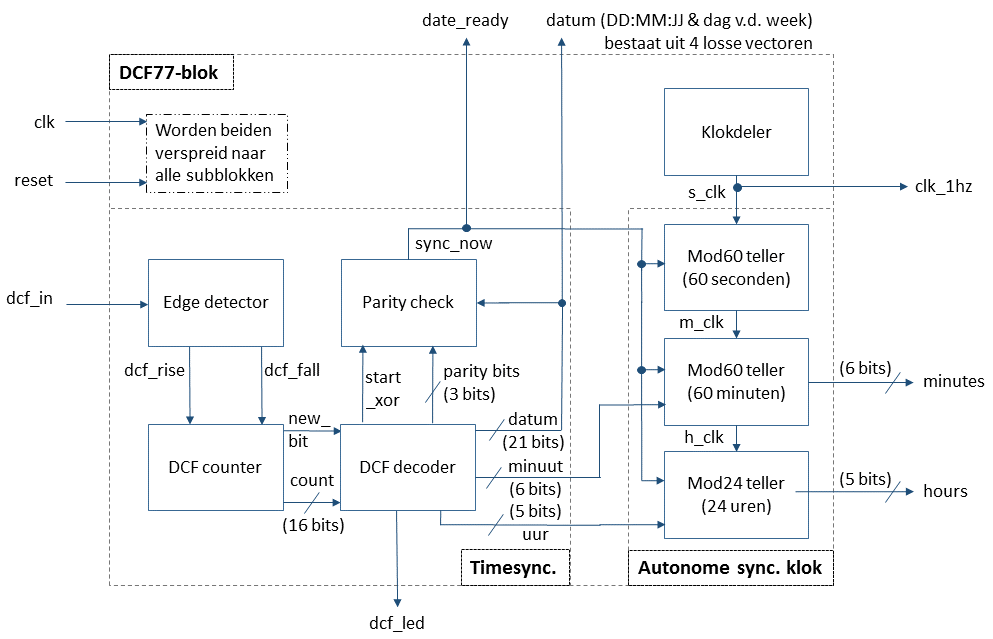
\includegraphics[keepaspectratio=true,scale=0.75]{Figuren/DCF77/Blokdiagram.png}
\caption{Verdeling van het DCF blok in subblokken}
\label{fig: dcf_subblokken}
\end{center}
\end{figure}